\documentclass{article}
\usepackage[margin=1.0in]{geometry}
\usepackage{amsmath, amsfonts, amssymb}
\usepackage{graphicx}
\usepackage{booktabs}
\usepackage{dirtytalk}
\graphicspath{{./images/}}
\renewcommand{\familydefault}{\sfdefault}

\title{Geospatial Big Data Analysis - Lab 4}
\author{
    Konstantinos Papadakis\\
    Student of MSc Data Science and Machine Learning - 03400149\\
    konstantinospapadakis@mail.ntua.gr
}
\date{\vspace{-5ex}}

\begin{document}

\maketitle

\begin{abstract}
    In this document we will discuss and evaluate a Recurrent Neural Network approach and a Self-Attention approach for classifying a selection of five categories from the UCF101 dataset.
\end{abstract}

\section{The Dataset}
The dataset is composed of the categories “CricketShot”, “PlayingCello”, “Punch”, “ShavingBeard” and “TennisSwing” of the UCF101 dataset. For each category there are 25 \emph{video groups} which are composed of, typically 7, \emph{video crops} of a single original video, so that the crops are short enough to be used for machine learning. Video groups with indices from 1 to 7 are part of the \emph{test set}, and video groups with indices from 8 to 25 are part of the \emph{training set}. We randomly sample 3 indices in \(\{8, \dots , 25\}\) and use the video groups with those indices as our \emph{validation set}.

\section{Classification}
We first perform feature extraction, using a single frame each time, with a 2D ResNet18 pre-trained on ImageNet and with its final linear layer removed and its weights frozen. This way each video is represented by a sequence of 512 dimensional vectors. We then examine two different approaches for sequence classification, an RNN approach and a self-attention approach. In both approaches we use architectures of similar sizes so that the results are comparable.

\subsection{RNN Approach}
In this approach we train a 2-layer GRU and pass its final output to a linear layer to perform classification. We used a hidden state size of 512 and a dropout with probability 0.1. The best model was achieved on epoch 17 (max epochs = 300, early stopping patience = 50). We notice that “CricketShot” has relatively low precision, and that “Punch” and “TennisSwing” have relatively low recall. The main source of this is the misclassification of “Punch” and “TennisSwing” samples as “CricketShot”. The reason for this could be that all three movements involve a throw-like motion of the arm.

\begin{table}[h]
    \label{clfrep:gru}
    \centering
    \begin{tabular}{lrrrr}
        \toprule
        & precision & recall & f1-score & support \\
        \midrule
        CricketShot & 0.86 & 0.98 & 0.91 & 49 \\
        PlayingCello & 1.00 & 0.98 & 0.99 & 44 \\
        Punch & 0.97 & 0.85 & 0.90 & 39 \\
        ShavingBeard & 0.98 & 1.00 & 0.99 & 43 \\
        TennisSwing & 0.96 & 0.92 & 0.94 & 49 \\
        \midrule
        accuracy &  &  & 0.95 & 224 \\
        macro avg & 0.95 & 0.94 & 0.95 & 224 \\
        weighted avg & 0.95 & 0.95 & 0.95 & 224 \\
        \bottomrule
    \end{tabular}
    \caption{Classification report of the GRU model}
\end{table}

\begin{figure}[h]
    \label{fig:confmat_gru}
    \centering
    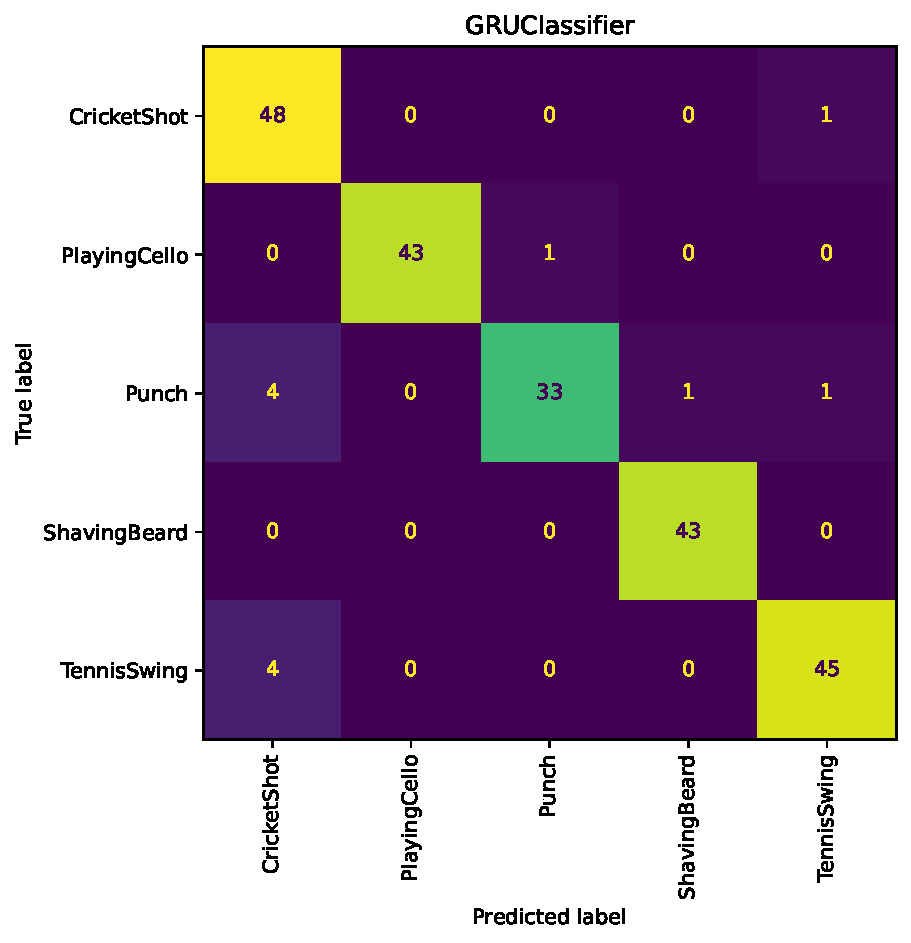
\includegraphics[scale=0.5]{./confusion_matrix_gru.pdf}
    \caption{Confusion matrix of the GRU model}
\end{figure}


\subsection{Self-Attention Approach}
In this approach we train a 2-layer Transformer Encoder where we take the maximum across the time dimension of the encoded sequence and then pass it to a linear layer for classification. The multihead self-attention layers have dimension 512 and 8 heads while the feedforward layers have inner layer size of 2048. Positional encoding is applied to the input before it is passed to the encoder. Dropout with probability 0.1 is performed between each layer. The best model was achieved on epoch \emph{2(!)} (max epochs = 300, early stopping patience = 50).  We notice that the confusion of “CricketShot”, “Punch” and “TennisSwing” still happens, but to a lesser degree. The Transformer model performed strictly better than the GRU model.

\begin{table}[h]
    \label{clfrep:transformer}
    \centering
    \begin{tabular}{lrrrr}
        \toprule
        & precision & recall & f1-score & support \\
        \midrule
        CricketShot & 0.94 & 1.00 & 0.97 & 49 \\
        PlayingCello & 1.00 & 1.00 & 1.00 & 44 \\
        Punch & 1.00 & 0.95 & 0.97 & 39 \\
        ShavingBeard & 0.98 & 1.00 & 0.99 & 43 \\
        TennisSwing & 1.00 & 0.96 & 0.98 & 49 \\
        \midrule
        accuracy &  &  & 0.98 & 224 \\
        macro avg & 0.98 & 0.98 & 0.98 & 224 \\
        weighted avg & 0.98 & 0.98 & 0.98 & 224 \\
        \bottomrule
    \end{tabular}
    \caption{Classification report of the Transformer model}
\end{table}

\begin{figure}[h]
    \label{fig:confmat_transformer}
    \centering
    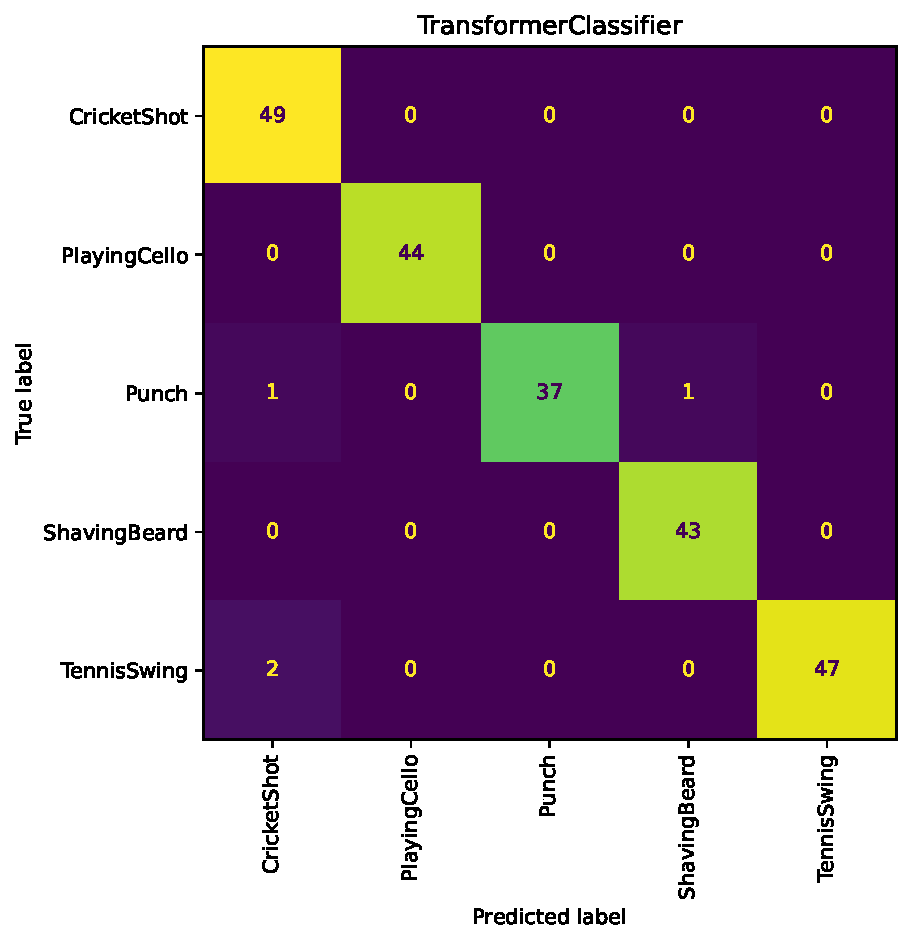
\includegraphics[scale=0.5]{./confusion_matrix_transformer.pdf}
    \caption{Confusion matrix of the Transformer model}
\end{figure}

\section{Questions}

\subsection{}
\say{Can bidirectional RNNs be used for online predicting on stream data?}

It is possible to use bidirectional RNNs for online predictions by simply calling the network on the current sequence at each time. This would be a lot more computationally intensive, since to get the outputs we would require a backward traversal of the entire sequence instead of just 1 forward step.

It is important though to note that \emph{if we use only the final element of the output sequence of the RNN}, then the backward traversal is wasted computation since we only utilize the zeroth hidden state which is a zero vector. Thus, in that case, there is no point in using a bidirectional RNN.

\subsection{}
\say{In your opinion, which is the most important classification metric in a security application?}

This depends on the severance of the consequences of a false negative. If the consequences are very severe, for example where human life is at stake, then recall is the most important metric. If on the other hand we don’t mind trading a few false negatives if this means having better precision, for example spam email detection, then a measure like F1 which balances between precision and recall could be more appropriate.

\subsection{}
\say{What can cause exploding gradients during RNN training? Recommend at least two ways with which such an issue can be resolved.}

See also Chapter 10 in \cite{Goodfellow-et-al-2016}.

The function composition employed by recurrent neural networks somewhat resembles matrix multiplication. We can think of the recurrence relation
\[h^{(t)} = W^\top h^{(t-1)}\]
as a very simple recurrent neural network lacking a nonlinear activation function, and lacking inputs x. This recurrence relation may be simplified to
\[h^{t} = \left( W^t \right)^\top h^{(0)}\]
and if \(W\) admits an eigendecomposition of the form
\[W = Q \Lambda Q^\top\]
with orthogonal \(Q\), the recurrence may be simplified further to
\[h^{(t)} = Q^\top \Lambda Q h^{(0)}\]
The eigenvalues are raised to the power of \(t\) causing eigenvalues with magnitude less than one to decay to zero and eigenvalues with magnitude greater than one to explode. Any component of \(h^{(0)}\) that is not aligned with the largest eigenvector will eventually be discarded.

% This problem is particular to recurrent networks. In the scalar case, imagine multiplying a weight \(w\) by itself many times. The product \(w^t\) will either vanish or explode depending on the magnitude of \(w\). However, if we make a non-recurrent network that has a different weight \(w^{(t)}\) at each time step, the situation is different. If the initial state is given by 1, then the state at time \(t\) is given by \(\prod_t w^{(t)}\). Suppose that the \(w^{(t)}\) values are generated randomly, independently from one another, with zero mean and variance \(v\). The variance of the product is \(O(v^n)\). To obtain some desired variance \(v^*\) we may choose the individual weights with variance \(v = \sqrt[n]{v^*}\). Very deep feedforward networks with carefully chosen scaling can thus avoid the vanishing and exploding gradient problem, as argued by Sussillo (2014).

One way to deal with exploding gradients is to clip the norm of the gradient just before the parameter update, that is 
\[\text{if}\ \lVert g \rVert > v\ \text{then}\ g \gets \frac{v}{\lVert g \rVert} g\]

Another way which is to use gated RNNs like LSTMs and GRUs, which are based on the idea of creating paths through time that have derivatives that neither vanish nor explode.

\bibliographystyle{IEEEtran}
\bibliography{refs}
\end{document}
